\documentclass[t, aspectratio=169]{beamer}
\usepackage[utf8]{inputenc}
\usepackage[T1]{fontenc}
\usepackage{amsthm,amsmath,amssymb}
\usepackage{tabularx}
\usepackage{booktabs}
\usepackage{array}
\usepackage[table]{xcolor}
\usepackage{lmodern}
\usepackage{graphicx}
\usepackage{tikz}
\usetikzlibrary{shapes.geometric, arrows.meta, positioning, calc}

% --- FONT SIZES ---
\setbeamerfont{frametitle}{size=\large}

% --- TIKZ STYLES ---
\tikzset{
    block_pink/.style={rectangle, draw, rounded corners, fill=pink!20, text width=3.5cm, text centered, minimum height=1.2cm},
    block_yellow/.style={rectangle, draw, rounded corners, fill=yellow!20, text width=3.5cm, text centered, minimum height=1.2cm},
    block_green/.style={rectangle, draw, rounded corners, fill=green!20, text width=3.5cm, text centered, minimum height=1.2cm},
    block_blue/.style={rectangle, draw, rounded corners, fill=blue!10, text width=3.5cm, text centered, minimum height=1.2cm},
    arrow/.style={-Latex, thick}
}

% --- MARGIN CONFIGURATION ---
\def\slideContentLeftMargin{0.5cm} 
\def\slideContentRightMargin{1cm}   
\def\hustHeaderHeight{1cm}        
\def\slideContentBotMargin{3.5cm}   

\usepackage[blue, 169]{beamerthemeHUST} 

\renewcommand{\titlePageTitleX}{-0.5cm}
\renewcommand{\titlePageTitleY}{-0.5cm}
\renewcommand{\hustTitleAlign}{\alignLeft} 
\renewcommand{\hustSubtitleAlign}{\alignLeft}
\renewcommand{\hustAuthorAlign}{\alignLeft}
\renewcommand{\hustInstAlign}{\alignLeft}

\title{HIGH-SPEED FPGA-BASED POST-PROCESSING ARCHITECTURE FOR CV-QKD SYSTEMS}
\subtitle{Information Reconciliation}
\author{Nguyen Minh Sang, Vu Quang Huy} 
\institute{Project Report}

\begin{document}
	
	% Title page
	\husttitlepage
	
	\begin{frame}[allowframebreaks]{Table of Contents}
		\tableofcontents[hideallsubsections]
	\end{frame}
	
	\resetPageCount  
	\showPageNumber  
	
	\useStyleHustFull
	\useThinBar 
	
	% =================================================================
	\section{Overview \& Objectives}
	% =================================================================
	
	\begin{frame}{Research Background}
        \textbf{Quantum Cryptography Context:}
        \begin{itemize}
            \item \textbf{Quantum Key Distribution (QKD):} Offers unconditional cryptographic security based on the laws of quantum mechanics, securing data against future quantum computer attacks.
            \vspace{0.8em}
            \item \textbf{The Bottleneck:} Free-Space Optical (FSO) channels (e.g., satellite links) experience severe and unpredictable Quantum Bit Error Rate (QBER) fluctuations.
            \vspace{0.8em}
            \item \textbf{The Post-Processing Challenge:} Extracting a consistent, error-free key from noisy raw quantum data is extremely computationally intensive, often causing severe throughput bottlenecks.
        \end{itemize}
	\end{frame}

	\begin{frame}{Project Objectives}
        \textbf{Core Goals:}
        \begin{itemize}
            \item \textbf{Hardware Acceleration:} Design a high-speed FPGA-based Post-Processing architecture to overcome computational bottlenecks.
            \vspace{0.8em}
            \item \textbf{Dynamic Adaptation:} Implement an autonomous \textit{Blind Reconciliation} protocol to dynamically handle wildly fluctuating QBER without wasting key rate on pre-estimation.
            \vspace{0.8em}
            \item \textbf{Platform Deployment:} Deploy and validate the architecture using a modern HW/SW Co-Design approach on the Gowin 138K Pro SoC (RISC-V + FPGA).
        \end{itemize}
	\end{frame}
	
	\begin{frame}{QKD Post-Processing Pipeline}
		\begin{center}
		% Hãy sửa "ten_file_anh_cua_ban.png" thành tên file ảnh thực tế của bạn
		\includegraphics[height=0.8\textheight]{Screenshot 2026-08-08 153742.png}
		\end{center}
	\end{frame}
	
	\begin{frame}{Literature Review: High-Speed QKD Post-Processing}
        \textbf{Review of Recent FPGA Accelerations:}
        \begin{itemize}
            \item \textbf{[2020] High-Speed Post-Processing in CV-QKD:} Demonstrated the necessity of FPGA acceleration for post-processing to meet real-time QKD demands, though rigid hardware structures limited flexibility against fluctuating quantum noise.
            \vspace{0.5em}
            \item \textbf{[2023] Acceleration of QC-LDPC Syndrome Encoding:} Focused on the transmitter side (Alice), significantly improving encoding throughput via highly parallelized FPGA pipelines.
            \vspace{0.5em}
            \item \textbf{[2023] Large-Scale FPGA-Based Privacy Amplification:} Achieved high-speed Toeplitz hashing to compress keys and remove leaked information. However, it highlighted that the primary latency bottleneck still remains in the \textit{Information Reconciliation} decoding step.
        \end{itemize}
	\end{frame}

	\begin{frame}{Literature Review: Rate-Compatible LDPC \& Blind Reconciliation}
        \textbf{Advancements in LDPC Construction:}
        \begin{itemize}
            \item \textbf{[2022] Rate-Compatible (RC) High-Throughput Scheme:} Addressed the need for multiple code rates using RC-LDPC to handle varying QBER, but required complex control logic and massive memory for routing.
            \vspace{0.5em}
            \item \textbf{Collaborative RC QC-LDPC (Extension \& Splitting):} Proposed profound mathematical models for rate compatibility, yet translating these complex matrix extensions efficiently into limited Block RAMs on mid-range FPGAs remains challenging.
            \vspace{0.5em}
            \item \textbf{Blind Reconciliation for FSO Satellites:} Introduced "Blind" protocols to avoid QBER pre-estimation in rapidly fluctuating Free-Space Optical channels. However, these methods often relied on random-based LDPC constructions that lack hardware-friendly, partially-parallel structures.
        \end{itemize}
	\end{frame}

	\begin{frame}{Existing Limitations in Current Research}
        \textbf{Key Limitations:}
        \begin{itemize}
            \item \textbf{Resource Exhaustion:} Multi-rate decoders require massive ROM tables or multiple instantiated matrices, rapidly depleting FPGA logic (LUT/BRAM).
            \vspace{0.8em}
            \item \textbf{Trapping Sets (Error Floors):} Low hardware precision (6-8 bit) quantizations inherently suffer from local minimums in Offset Min-Sum decoding, preventing convergence even at low QBER.
            \vspace{0.8em}
            \item \textbf{Latency Overhead:} Fixed decoding iterations (e.g., waiting for $MAX\_ITER$) and the need for QBER pre-estimation waste valuable key rate and increase processing delays.
        \end{itemize}
	\end{frame}

	\begin{frame}{Our Proposed Solution (Gowin 138K Pro)}
        \textbf{System Enhancements:}
        \begin{itemize}
            \item \textbf{HW/SW Co-Design:} RISC-V firmware seamlessly orchestrates a dynamic \textit{Blind Reconciliation FSM} to natively handle fluctuating QBER without prior estimation.
            \vspace{0.8em}
            \item \textbf{High-Precision Datapath (12-12-14 bit):} By utilizing Gowin 138K B-SRAMs, the system eliminates hardware-induced trapping sets, enabling perfect convergence.
            \vspace{0.8em}
            \item \textbf{Zero-Overhead Adaptation:} A unified Rate 1/2 matrix utilizing \textit{Hard-Puncturing} for multi-rate support, integrated with \textit{Early Termination} for maximum throughput.
        \end{itemize}
	\end{frame}
	
	\begin{frame}{System Overview}
		\textbf{Target Platform:} Tang Mega 138K Pro (Gowin GW5AST-138 SoC).
        
        \vspace{0.5em}
		\textbf{Architectural Approach: Hardware/Software Co-Design.}
		\begin{itemize}
			\item \textbf{RISC-V AE350 (Software):} Handles protocol orchestration, DMA data buffering, dynamic syndrome padding, and Blind Reconciliation control.
			\item \textbf{FPGA Fabric (Hardware):} Accelerates computationally heavy mathematical operations (LDPC Decoding).
		\end{itemize}
        
        \vspace{0.5em}
        \textbf{Core Cryptographic Stages:}
        \begin{itemize}
            \item Utilizes an IEEE 802.16e QC-LDPC Decoder for Information Reconciliation.
        \end{itemize}
	\end{frame}
	
	\begin{frame}{Key Technical Advancements}
		\begin{itemize}
			\item \textbf{High-Precision Quantization (12-12-14 bit):} Eliminated Trapping Sets completely.
			\item \textbf{Dynamic Blind Reconciliation FSM:} Automatic rate scaling for fluctuating QBER.
			\item \textbf{Early Termination Logic:} Halts iterations immediately upon parity check success.
			\item \textbf{Hard Puncturing Multiplexing:} Zero-overhead multi-rate adaptation.
		\end{itemize}
	\end{frame}

	% =================================================================
	\section{HW/SW Co-Design Architecture}
	% =================================================================
	\useStyleLogoOnly 
	\useThickBar      
	
	\begin{frame}{Proposed HW/SW Co-Design Architecture}
		\begin{center}
		\resizebox{0.9\textwidth}{!}{%
		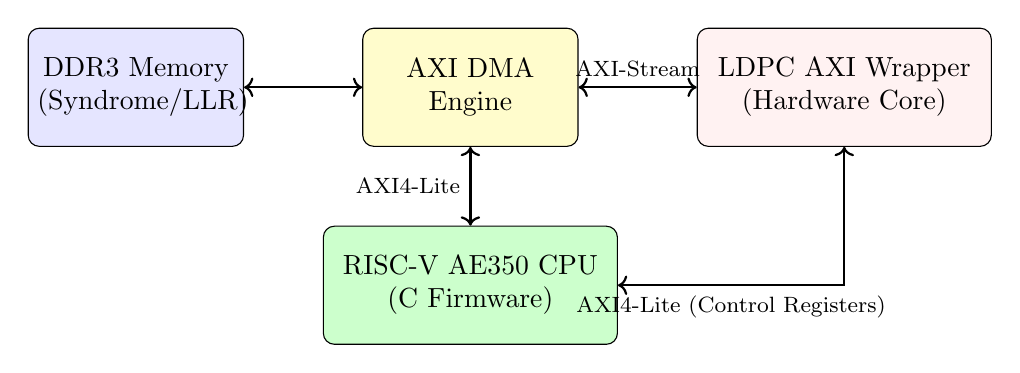
\begin{tikzpicture}[node distance=1cm and 1.5cm]
			\node (ddr) [block_blue, text width=2.5cm, minimum height=1.5cm] {DDR3 Memory\\(Syndrome/LLR)};
			\node (dma) [block_yellow, right=of ddr, text width=2.5cm, minimum height=1.5cm] {AXI DMA\\Engine};
			\node (wrapper) [block_pink, right=of dma, text width=3.5cm, minimum height=1.5cm] {LDPC AXI Wrapper\\(Hardware Core)};
            \node (riscv) [block_green, below=of dma, text width=3.5cm, minimum height=1.5cm] {RISC-V AE350 CPU\\(C Firmware)};
			
			\draw [arrow, <->] (ddr) -- (dma);
			\draw [arrow, <->] (dma) -- node[above]{\footnotesize AXI-Stream} (wrapper);
            \draw [arrow, <->] (riscv) -- node[left]{\footnotesize AXI4-Lite} (dma);
            \draw [arrow, <->] (riscv) -| node[below, pos=0.25]{\footnotesize AXI4-Lite (Control Registers)} (wrapper);
		\end{tikzpicture}%
		}
		\end{center}
	\end{frame}
	
	% =================================================================
	\section{LDPC Core Design}
	% =================================================================
	\useStyleHustFull
	\useThinBar 
	
	\begin{frame}{Technical Specifications}
		\begin{table}[]
        \centering
        \renewcommand{\arraystretch}{1.2}
        \begin{tabular}{ll}
        \hline
        \rowcolor{blue!10} \textbf{Parameter} & \textbf{Specification} \\ \hline
        Base Matrix Standard & IEEE 802.16e (WiMAX) \\
        Block Length (N) & 2304 bits \\
        Expansion Factor ($Z_c$) & 96 \\
        Supported Code Rates & 1/2, 2/3, 3/4 (Dynamic Switching) \\
        Decoding Algorithm & Offset Min-Sum (OMS) \\
        Max Iterations & 32 (With Early Termination capability) \\
        Hardware Architecture & Partially Parallel ($Z_c$ nodes processed per clock) \\ \hline
        \end{tabular}
        \end{table}
	\end{frame}

	\begin{frame}{High-Precision Quantization Strategy}
        \vspace{0.5em}
		\begin{itemize}
			\item \textbf{Log-Likelihood Ratio (LLR) Input:} \textbf{12-bit} Signed.
			\item \textbf{Check-to-Variable (C2V) Messages:} \textbf{12-bit} Signed.
			\item \textbf{Variable-to-Check (V2C) Messages:} \textbf{14-bit} Signed.
		\end{itemize}

        \vspace{1em}

	\end{frame}

	\begin{frame}{Zero-Overhead Rate Adaptation}
		\textbf{Challenge:} Traditional Multi-Rate LDPC decoders require instantiating multiple distinct hardware cores or storing massive ROM tables, depleting FPGA LUTs.
		
		\vspace{1em}
		\textbf{Solution: Hard Puncturing Multiplexing}
		\begin{itemize}
			\item Implemented a unified, single-core architecture based exclusively on the \textbf{Rate 1/2 mother matrix}.
			\item Developed a dynamic Hard Puncturing Multiplexer situated right before the decoder input.
			\item Depending on the RISC-V control signal (\texttt{code\_rate}), the MUX artificially gates specific blocks of incoming LLRs to 0, dynamically simulating Rate 2/3 or 3/4 without changing the hardware matrix.
		\end{itemize}
	\end{frame}

	\begin{frame}{Partially Parallel Architecture \& Compare Tree}
		\textbf{Challenge:} A fully parallel instantiation of an $N=2304$ LDPC matrix would require an astronomical number of wiring interconnects, leading to severe routing congestion and inevitable timing closure failures.
		
		\vspace{1em}
		\textbf{Innovative Solutions:}
		\begin{itemize}
			\item \textbf{Partially Parallel Processing:} Instead of computing all nodes simultaneously, the hardware processes exactly one sub-matrix block ($Z_c = 96$ nodes) per clock cycle.
            \item \textbf{Inlined VNU Logic:} Variable Node Updates ($LLR = LLR + V2C$) are embedded directly within the pipeline register stages, saving instantiation overhead.
			\item \textbf{Min-Tree Comparator (CNU):} The Check Node Units in the Offset Min-Sum algorithm require finding the 1st and 2nd minimum values among heavily quantized incoming signals. By deploying a pipelined binary Compare-Tree, the logic depth was dramatically shortened.
		\end{itemize}
	\end{frame}

	\begin{frame}{Throughput Optimization via Early Termination}
		\textbf{The Latency Problem:} The Belief Propagation algorithm iteratively refines probabilities up to a worst-case boundary of $MAX\_ITER = 32$. However, in high-quality optical links ($QBER < 2\%$), the matrix often resolves all errors within the first 5 to 8 iterations.
		
		\vspace{1em}
		\textbf{The Smart Halting Mechanism:}
		\begin{itemize}
			\item Integrated a high-speed parity evaluation tree (\texttt{all\_layers\_parity\_ok}) inside the Check Node Unit.
			\item Modified the core FSM in the \texttt{LAYER\_WRITE} state to continuously monitor this flag.
			\item If the mathematical condition is completely satisfied before reaching $MAX\_ITER$, the FSM short-circuits the iterative loop and jumps directly to the \texttt{OUTPUT\_RES} state to flush the clean key out.
		\end{itemize}
	\end{frame}

    % =================================================================
	\section{Blind Reconciliation FSM}
	% =================================================================
	\useStyleLogoOnly 
	\useThickBar 

	\begin{frame}{Multi-Rate Blind Reconciliation Workflow}
		\begin{center}
		\resizebox{0.75\textwidth}{!}{%
		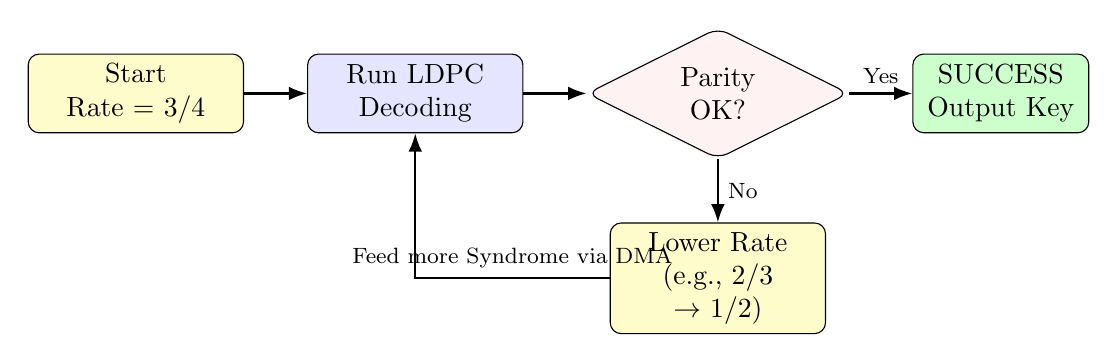
\begin{tikzpicture}[node distance=0.8cm and 0.8cm]
			\node (start) [block_yellow, text width=2.5cm, minimum height=1cm] {Start\\Rate = 3/4};
			\node (decode) [block_blue, right=of start, text width=2.5cm, minimum height=1cm] {Run LDPC\\Decoding};
			\node (check) [block_pink, right=of decode, diamond, aspect=2, text width=2cm, minimum height=1cm, inner sep=0pt] {Parity\\OK?};
            \node (success) [block_green, right=of check, text width=2cm, minimum height=1cm] {SUCCESS\\Output Key};
            \node (fail) [block_yellow, below=of check, text width=2.5cm, minimum height=1cm] {Lower Rate\\(e.g., 2/3 $\rightarrow$ 1/2)};
			
			\draw [arrow] (start) -- (decode);
			\draw [arrow] (decode) -- (check);
			\draw [arrow] (check) -- node[above]{\footnotesize Yes} (success);
            \draw [arrow] (check) -- node[right]{\footnotesize No} (fail);
            \draw [arrow] (fail) -| node[above, pos=0.25]{\footnotesize Feed more Syndrome via DMA} (decode);
		\end{tikzpicture}%
		}
		\end{center}

        \vspace{0.5em}
        \textbf{The "Blind" Solution (Zero-Communication Overhead):} 
        \begin{itemize}
            \item System  attempts to decode using Rate 3/4 to maximize Secure Key Rate.
            \item If LDPC fails, it fires \texttt{ir\_fail} to the RISC-V CPU.
            \item RISC-V autonomously down-shifts the rate (to 2/3, then 1/2), injects more Syndrome bits via DMA, and resumes decoding locally.
        \end{itemize}
	\end{frame}
	
	% =================================================================
	\section{Simulation Results \& Verification}
	% =================================================================
	\useStyleHustFull
	\useThinBar 

	\begin{frame}{Bit-Accurate Golden Model Verification}
		\begin{itemize}
            \item \textbf{Python Golden Model (\texttt{hw\_exact\_sim.py}):} Developed a custom, bit-accurate Python simulator mirroring the hardware's architecture, including 12-bit fixed-point thresholds and Hard Puncturing logic.
            \item \textbf{Cross-Verification:} Verilog RTL dumps are aggressively cross-referenced against Python outputs to guarantee mathematical correctness.
        \end{itemize}
	\end{frame}

	\begin{frame}{Testbench Results \& Verification}
		\begin{table}[]
        \centering
        \renewcommand{\arraystretch}{1.2}
        \begin{tabular}{ccccc}
        \hline
        \rowcolor{blue!10} \textbf{Block ID} & \textbf{Initial Errors} & \textbf{QBER} & \textbf{Final Errors} & \textbf{Status} \\ \hline
        0 & 89 & 3.86\% & \textbf{0} & \textcolor{green!60!black}{\textbf{SUCCESS}} \\
        1 & 76 & 3.30\% & 0 & \textcolor{green!60!black}{\textbf{SUCCESS}} \\
        2 & 87 & 3.78\% & 0 & \textcolor{green!60!black}{\textbf{SUCCESS}} \\
        3 & 79 & 3.43\% & 0 & \textcolor{green!60!black}{\textbf{SUCCESS}} \\
        4 & 91 & 3.95\% & 33 & \textcolor{red}{\textbf{FAILED (Blind Fallback)}} \\
        5 & 194 & 8.42\% & \textbf{0} & \textcolor{green!60!black}{\textbf{SUCCESS (Post-Fallback)}} \\ \hline
        \end{tabular}
        \end{table}
	\end{frame}

	\begin{frame}{Simulation Analysis: The Nature of Trapping Sets}
        \begin{itemize}
            
            \vspace{0.8em}
            \item \textbf{Topological Stubbornness (Block 4):} 
            Block 4 has 91 errors (3.95\% QBER), almost identical to Block 0. However, even when running at \textbf{Rate 1/2}, it still fails with 33 residual errors. This proves that Trapping Sets are driven by the \textit{specific spatial distribution} of errors aligning with short cycles in the Tanner Graph, rendering even high-precision hardware helpless.

            \vspace{0.8em}
            \item \textbf{High-Noise Resilience (Block 5):} 
            Block 5 has a massive 194 errors (8.42\% QBER), double that of Block 4. Yet, it perfectly converges to 0 errors at Rate 1/2! This demonstrates that the 12-bit OMS decoder is extremely powerful against random noise, highlighting that the failure of Block 4 was strictly a topological trap, not a Shannon limit or hardware capacity issue.
        \end{itemize}
	\end{frame}

    % =================================================================
	\section{Future Works}
	% =================================================================
	\useStyleLogoOnly 
	\useThickBar 

    \begin{frame}{Future Works}
		\begin{enumerate}
            \item \textbf{Privacy Amplification (PA) Integration:} 
            \begin{itemize}
                \item Integrate the Toeplitz Hashing Core (\texttt{pa\_toeplitz\_hash.v}) directly after the LDPC decoder to compress the reconciled key and remove information leaked to Eve.
            \end{itemize}
            
            \vspace{0.8em}
            \item \textbf{Transmitter-Side Syndrome Generation (Alice):} 
            \begin{itemize}
                \item Establish a robust communication link (Ethernet or UART) between Alice and the Tang Mega 138K Pro (Bob) to transmit Syndrome data in real-time.
            \end{itemize}
            
            \vspace{0.8em}
            \item \textbf{Gowin Board Deployment:} 
            \begin{itemize}
                \item Flash the RISC-V C-firmware onto the physical AE350 core.
                \item Validate the End-to-End throughput on actual hardware.
            \end{itemize}
        \end{enumerate}
	\end{frame}

	\hustthankyou
	
\end{document}